% Options for packages loaded elsewhere
% Options for packages loaded elsewhere
\PassOptionsToPackage{unicode}{hyperref}
\PassOptionsToPackage{hyphens}{url}
\PassOptionsToPackage{dvipsnames,svgnames,x11names}{xcolor}
%
\documentclass[
]{article}
\usepackage{xcolor}
\usepackage{amsmath,amssymb}
\setcounter{secnumdepth}{-\maxdimen} % remove section numbering
\usepackage{iftex}
\ifPDFTeX
  \usepackage[T1]{fontenc}
  \usepackage[utf8]{inputenc}
  \usepackage{textcomp} % provide euro and other symbols
\else % if luatex or xetex
  \usepackage{unicode-math} % this also loads fontspec
  \defaultfontfeatures{Scale=MatchLowercase}
  \defaultfontfeatures[\rmfamily]{Ligatures=TeX,Scale=1}
\fi
\usepackage{lmodern}
\ifPDFTeX\else
  % xetex/luatex font selection
\fi
% Use upquote if available, for straight quotes in verbatim environments
\IfFileExists{upquote.sty}{\usepackage{upquote}}{}
\IfFileExists{microtype.sty}{% use microtype if available
  \usepackage[]{microtype}
  \UseMicrotypeSet[protrusion]{basicmath} % disable protrusion for tt fonts
}{}
\makeatletter
\@ifundefined{KOMAClassName}{% if non-KOMA class
  \IfFileExists{parskip.sty}{%
    \usepackage{parskip}
  }{% else
    \setlength{\parindent}{0pt}
    \setlength{\parskip}{6pt plus 2pt minus 1pt}}
}{% if KOMA class
  \KOMAoptions{parskip=half}}
\makeatother
% Make \paragraph and \subparagraph free-standing
\makeatletter
\ifx\paragraph\undefined\else
  \let\oldparagraph\paragraph
  \renewcommand{\paragraph}{
    \@ifstar
      \xxxParagraphStar
      \xxxParagraphNoStar
  }
  \newcommand{\xxxParagraphStar}[1]{\oldparagraph*{#1}\mbox{}}
  \newcommand{\xxxParagraphNoStar}[1]{\oldparagraph{#1}\mbox{}}
\fi
\ifx\subparagraph\undefined\else
  \let\oldsubparagraph\subparagraph
  \renewcommand{\subparagraph}{
    \@ifstar
      \xxxSubParagraphStar
      \xxxSubParagraphNoStar
  }
  \newcommand{\xxxSubParagraphStar}[1]{\oldsubparagraph*{#1}\mbox{}}
  \newcommand{\xxxSubParagraphNoStar}[1]{\oldsubparagraph{#1}\mbox{}}
\fi
\makeatother


\usepackage{longtable,booktabs,array}
\usepackage{calc} % for calculating minipage widths
% Correct order of tables after \paragraph or \subparagraph
\usepackage{etoolbox}
\makeatletter
\patchcmd\longtable{\par}{\if@noskipsec\mbox{}\fi\par}{}{}
\makeatother
% Allow footnotes in longtable head/foot
\IfFileExists{footnotehyper.sty}{\usepackage{footnotehyper}}{\usepackage{footnote}}
\makesavenoteenv{longtable}
\usepackage{graphicx}
\makeatletter
\newsavebox\pandoc@box
\newcommand*\pandocbounded[1]{% scales image to fit in text height/width
  \sbox\pandoc@box{#1}%
  \Gscale@div\@tempa{\textheight}{\dimexpr\ht\pandoc@box+\dp\pandoc@box\relax}%
  \Gscale@div\@tempb{\linewidth}{\wd\pandoc@box}%
  \ifdim\@tempb\p@<\@tempa\p@\let\@tempa\@tempb\fi% select the smaller of both
  \ifdim\@tempa\p@<\p@\scalebox{\@tempa}{\usebox\pandoc@box}%
  \else\usebox{\pandoc@box}%
  \fi%
}
% Set default figure placement to htbp
\def\fps@figure{htbp}
\makeatother





\setlength{\emergencystretch}{3em} % prevent overfull lines

\providecommand{\tightlist}{%
  \setlength{\itemsep}{0pt}\setlength{\parskip}{0pt}}



 


\makeatletter
\@ifpackageloaded{caption}{}{\usepackage{caption}}
\AtBeginDocument{%
\ifdefined\contentsname
  \renewcommand*\contentsname{Table of contents}
\else
  \newcommand\contentsname{Table of contents}
\fi
\ifdefined\listfigurename
  \renewcommand*\listfigurename{List of Figures}
\else
  \newcommand\listfigurename{List of Figures}
\fi
\ifdefined\listtablename
  \renewcommand*\listtablename{List of Tables}
\else
  \newcommand\listtablename{List of Tables}
\fi
\ifdefined\figurename
  \renewcommand*\figurename{Figure}
\else
  \newcommand\figurename{Figure}
\fi
\ifdefined\tablename
  \renewcommand*\tablename{Table}
\else
  \newcommand\tablename{Table}
\fi
}
\@ifpackageloaded{float}{}{\usepackage{float}}
\floatstyle{ruled}
\@ifundefined{c@chapter}{\newfloat{codelisting}{h}{lop}}{\newfloat{codelisting}{h}{lop}[chapter]}
\floatname{codelisting}{Listing}
\newcommand*\listoflistings{\listof{codelisting}{List of Listings}}
\makeatother
\makeatletter
\makeatother
\makeatletter
\@ifpackageloaded{caption}{}{\usepackage{caption}}
\@ifpackageloaded{subcaption}{}{\usepackage{subcaption}}
\makeatother
\usepackage{bookmark}
\IfFileExists{xurl.sty}{\usepackage{xurl}}{} % add URL line breaks if available
\urlstyle{same}
\hypersetup{
  pdftitle={R Basics},
  pdfauthor={Dr.~Eric Friedlander},
  colorlinks=true,
  linkcolor={blue},
  filecolor={Maroon},
  citecolor={Blue},
  urlcolor={Blue},
  pdfcreator={LaTeX via pandoc}}


\title{R Basics}
\usepackage{etoolbox}
\makeatletter
\providecommand{\subtitle}[1]{% add subtitle to \maketitle
  \apptocmd{\@title}{\par {\large #1 \par}}{}{}
}
\makeatother
\subtitle{Lecture 1}
\author{Dr.~Eric Friedlander}
\date{}
\begin{document}
\maketitle


\subsection{Before we start\ldots{}}\label{before-we-start}

\begin{itemize}
\tightlist
\item
  Make sure you have done the following:

  \begin{itemize}
  \tightlist
  \item
    Downloaded and installed R
  \item
    Downloaded and installed Positron (or R Studio)
  \item
    Created a Gemini Pro AI account (free for students)
  \end{itemize}
\end{itemize}

\section{Introduction to R}\label{introduction-to-r}

\subsection{What is R?}\label{what-is-r}

\begin{itemize}
\tightlist
\item
  R is a statistical programming language

  \begin{itemize}
  \tightlist
  \item
    Inspired by the S programming language developed at Bell Labs in the
    1970s
  \item
    Created by Ross Ihaka and Robert Gentleman at the University of
    Auckland, New Zealand in the early 1990s for teaching statistics
  \item
    Now one of the most popular programming languages for data science
    and statistics
  \end{itemize}
\item
  R is free and open source

  \begin{itemize}
  \tightlist
  \item
    Anyone can download and use R for free
  \item
    Anyone can contribute to the development of R and its packages
  \end{itemize}
\end{itemize}

\subsection{R is not the same as R Studio, R Markdown, or
Positron}\label{r-is-not-the-same-as-r-studio-r-markdown-or-positron}

\begin{itemize}
\tightlist
\item
  R is the programming language
\item
  R Studio (now Positron) is an integrated development environment (IDE)
  for R

  \begin{itemize}
  \tightlist
  \item
    Provides a user-friendly interface for writing and running R code
  \end{itemize}
\end{itemize}

\begin{figure}[H]

{\centering \pandocbounded{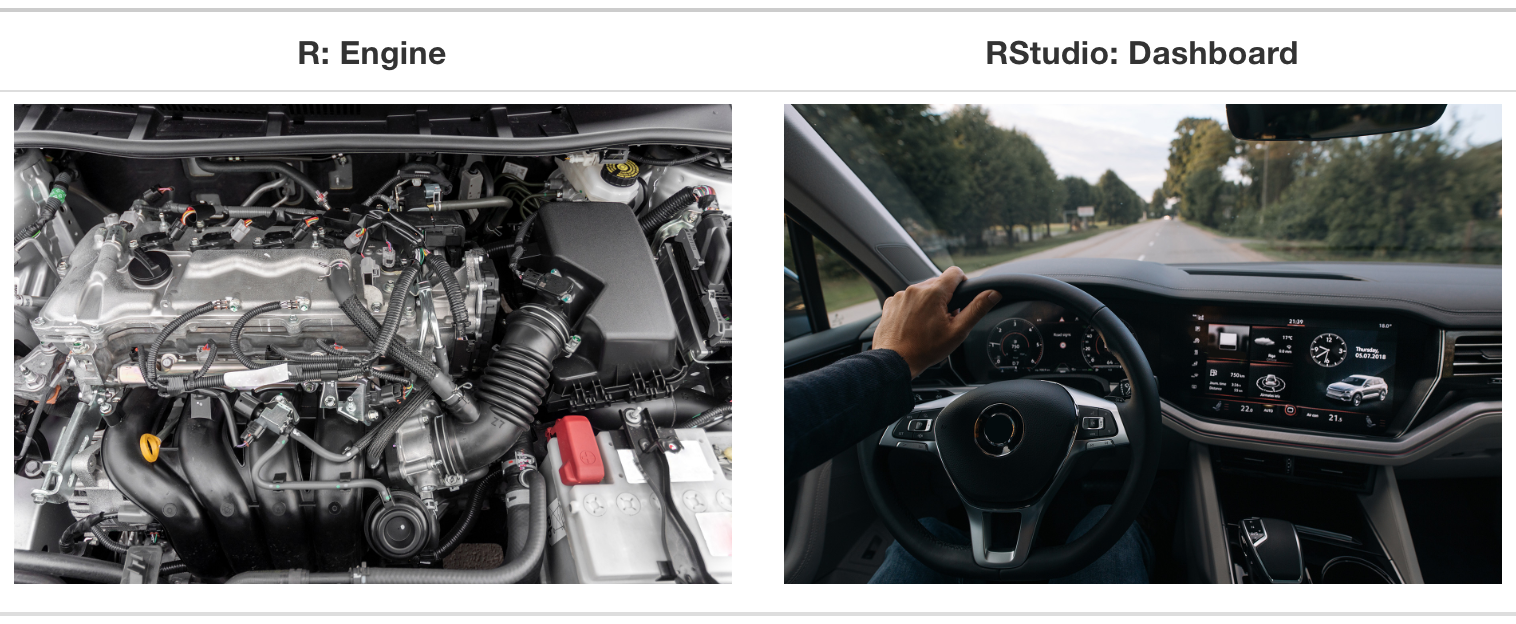
\includegraphics[keepaspectratio]{images/r_vs_rstudio_1.png}}

}

\caption{Source:
\href{https://moderndive.com/1-getting-started.html}{Statistical
Inference via Data Science}}

\end{figure}%

\section{Working with R}\label{working-with-r}

\subsection{Writing Scripts in R}\label{writing-scripts-in-r}

\begin{itemize}
\tightlist
\item
  Let's open up a script and run some R code!

  \begin{itemize}
  \tightlist
  \item
    Running R from the console
  \item
    Running R from a script file
  \end{itemize}
\end{itemize}

\subsection{R Packages}\label{r-packages}

\begin{itemize}
\tightlist
\item
  R has a rich ecosystem of packages that extend its functionality

  \begin{itemize}
  \tightlist
  \item
    You can install packages using
    \texttt{install.packages("package\_name")} (only do this once)
  \item
    Load packages into your R session using
    \texttt{library(package\_name)} (do this every time you start a new
    R session)
  \end{itemize}
\item
  An important package for this class:

  \begin{itemize}
  \tightlist
  \item
    \texttt{tidyverse}: A collection of packages for data manipulation,
    visualization, and modeling

    \begin{itemize}
    \tightlist
    \item
      \texttt{ggplot2}: A package for creating graphics using the
      Grammar of Graphics
    \item
      \texttt{dplyr}: A package for data manipulation
    \end{itemize}
  \end{itemize}
\item
  Let's install and load \texttt{tidyverse}
\end{itemize}

\subsection{Palmer Penguins Dataset}\label{palmer-penguins-dataset}

\begin{itemize}
\tightlist
\item
  Install the \texttt{palmerpenguins} package
\item
  Contains dataset on the famous Palmer Penguins: penguin species,
  island in Palmer Archipelago, size (flipper length, body mass, bill
  dimensions), and sex.
\item
  Explore more with \texttt{?penguins}
\end{itemize}

\subsection{Important Vocabulary}\label{important-vocabulary}

\begin{itemize}
\tightlist
\item
  \textbf{Data frame}: A table-like structure in R that holds data
  (\texttt{penguins})

  \begin{itemize}
  \tightlist
  \item
    In the \texttt{tidyverse} data frames are referred to as
    \texttt{tibbles}
  \end{itemize}
\item
  \textbf{Variable}: is a quantity, quality, or property that you can
  measure (e.g.~\texttt{species}, \texttt{bill\_length\_mm},
  \texttt{island})
\item
  \textbf{Observation} or \textbf{Data point}: a single object that has
  been measured (e.g.~one of the penguins in the data set)
\item
  \textbf{Value}: the entry for a particular variable and observation
  (e.g.~for the first penguin, the value of \texttt{species} is
  ``Adelie'', the value of \texttt{bill\_length\_mm} is 39.1)
\item
  \textbf{Tabular Data}: data organized in rows and columns (like a
  spreadsheet or data frame)
\item
  \textbf{Tidy Data}: tabular data where each observation is a row, each
  variable is a column, and each type of observational unit forms a
  table
\end{itemize}

\subsection{\texorpdfstring{Taking a quick look at
\texttt{penguins}}{Taking a quick look at penguins}}\label{taking-a-quick-look-at-penguins}

\begin{itemize}
\tightlist
\item
  \texttt{glimpse} gives a quick overview of the data frame
\item
  \texttt{head} shows the first few rows of the data frame
\item
  \texttt{tail} shows the last few rows of the data frame
\end{itemize}

\section{Wrap up}\label{wrap-up}

\subsection{Do Next}\label{do-next}

\begin{enumerate}
\def\labelenumi{\arabic{enumi}.}
\tightlist
\item
  Read the Introduction of
  \href{https://r4ds.had.co.nz/introduction.html}{R for Data Science}
\item
  Post any question you have to the HW channel in our Team.
\item
  Move on to Lecture 02.
\end{enumerate}




\end{document}
